\section{Linear Magnetoresistance in Na$_3$Bi with a High Chemical Potential}
\label{sec:na3bi:lmr}


Na$_3$Bi belongs to the space group P6$_3$/mmc and its lattice parameters are a = 5.448 $\rm{\AA}$ and c = 9.655 $\rm{\AA}$. It has a simple crystal structure with three distinct crystallographic sites: Na(1), Na(2), and Bi. It consists of Na(1)-Bi honeycomb layers stacked along the c axis, with Na(2) between the layers. Our first attempt to grow Na$_3$Bi crystals by slowly cooling a stoichiometric melt resulted in crystals with a lot of Na vacancies. As a result, they are mixed with the superconducting NaBi phase. To suppress these defects, we then used Na-rich compositions (90$\%$ and 95$\%$) and the flux-grow method \cite{Kushwaha}. We have obtained high-quality Na$_3$Bi crystals whose structure has been confirmed by X-ray diffraction (the lattice structure is sketched in Fig. \ref{figR}C). The crystals are deep purple and in an elongated hexagonal shape as shown in the inset of Fig. \ref{figR}A. Their largest facets are normal to the $c$-axis (001). Na$_3$Bi crystals are very fragile in any amount of water or oxygen. We find that they can be easily oxidized completely within 30 seconds in exposure to air. This has been a large obstacle to our sample mounting process. To protect the sample from any oxidization, we need to attach the contacts to the crystals with Ag epoxy inside an Ar glovebox and then cover the sample with paratone oil and seal it. Only after all these steps, we can safely load the sample into the cryostat (see the details in previous chapters). The resistance v.s. temperature curve (Fig. \ref{figR}A) of Na$_3$Bi shows a metallic behavior with the 4K resisitivity ranging from 1.72 to 87 $\mu\Omega$cm. Fig. \ref{figR}B shows the Hall effect which is linear and $n$-type. Fig. \ref{figR}A also indicates a nearly $T$-independent Hall coefficient $R_H = \rho_{yx}/B$ ($\bf\hat{x}||I$ and $\bf\hat{z}||\hat{c}$, where $\bf I$ is the current). We have measured several different batches of the crystals. Among them, Batch B and C were not annealed, while Batch G was annealed for one month. 

The typical MR curves of Na$_3$Bi at selected angles are shown in Figure \ref{figR}C. The tilt angle $\theta$ is between $\bf\hat{c}$ and the field ${\bf H}={\bf B}/\mu_0$, with $\mu_0$ the vacuum permeability). Here $\theta$ is defined as the angle between $\bf B$ and the $c$-axis of the sample. The current flows within the $a-b$ plane. The current and $\bf B$ are parallel when $\theta \equiv 90^\circ$. The MR profiles are linear in all angles, and their MR ratios reach the maximum at $\theta \equiv 0^\circ$ while decreasing with $\bf H$ tilted into the $a$-$b$ plane ($\theta\to 90^\circ$). 

\begin{figure}[!htbp]
  \begin{center}
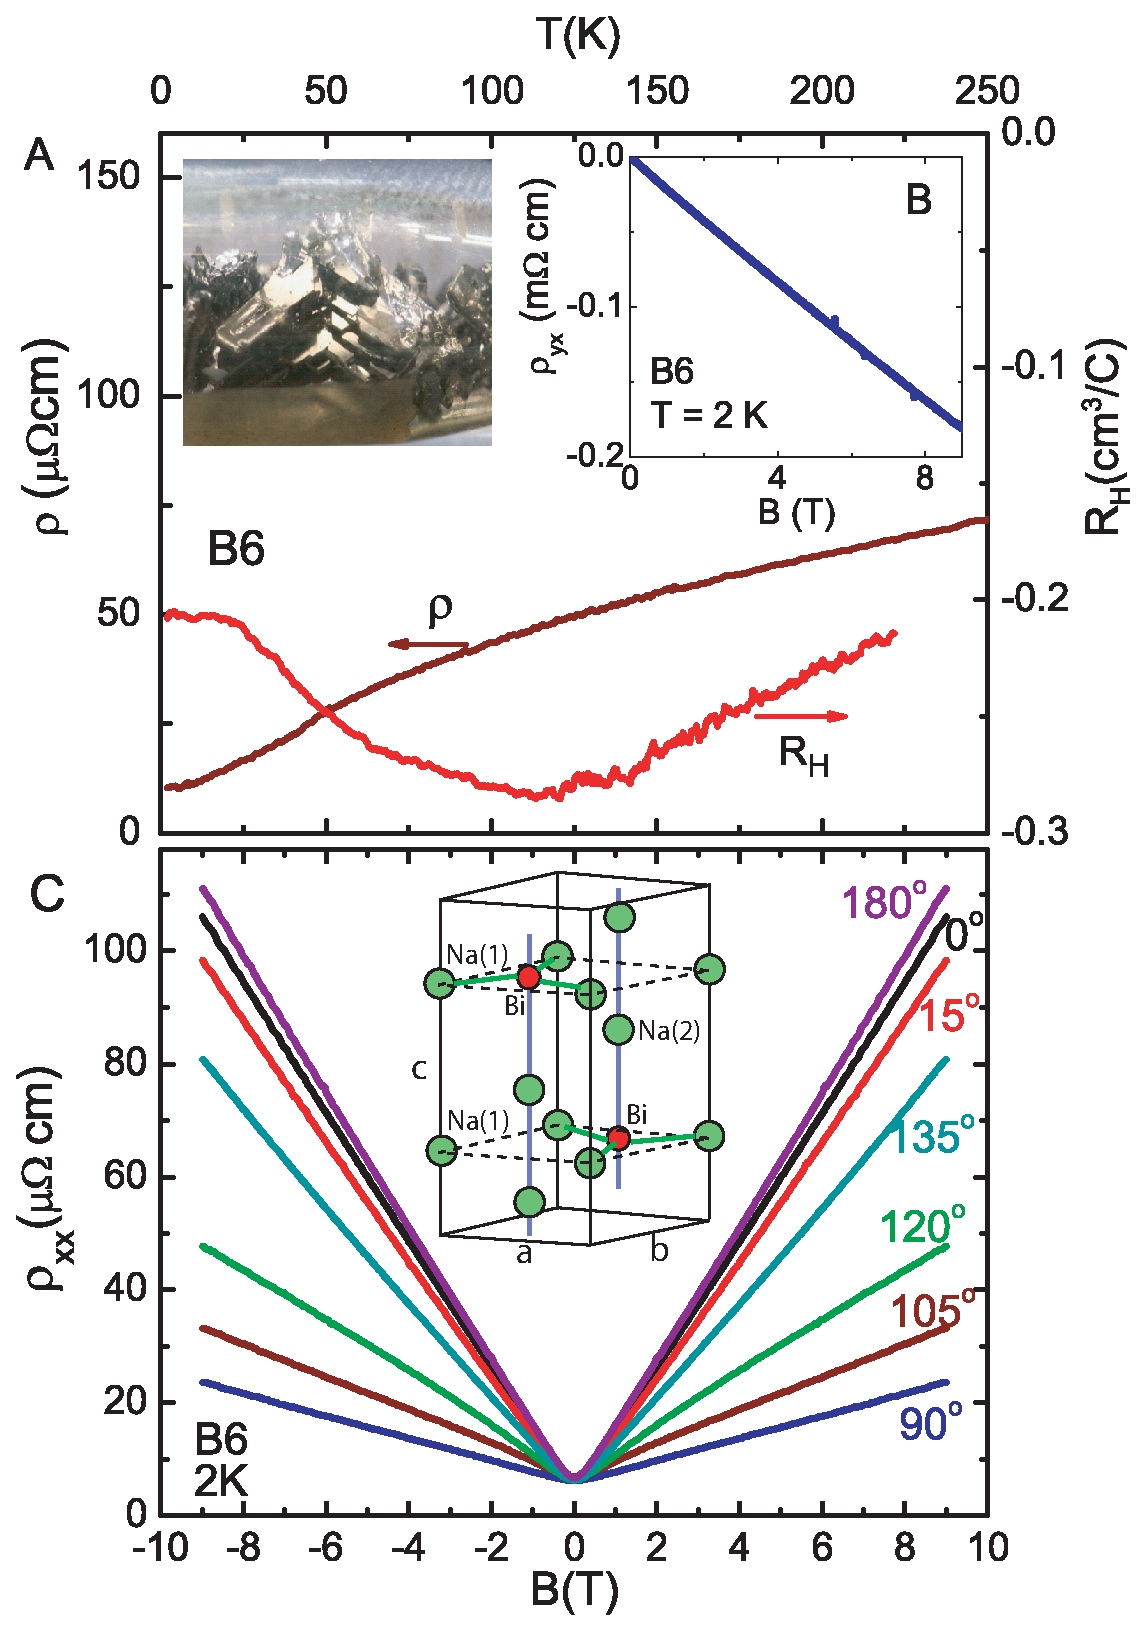
\includegraphics[width=0.8\linewidth]{ch-na3bi/figures/FigRMRA}
\caption{\label{figR}
Magnetotransport in Na$_3$Bi. Panel A: The zero-field resistivity $\rho$ and the Hall coefficient $R_H$ v.s. $T$ (measured with $\bf H||c$). Inset shows the crystals sealed in a vial. The largest facet is normal to $\bf\hat{c}$. Panel (B) shows the Hall resistivity $\rho_{yx}$ v.s. $B$ measured at 2 K in Sample B6.
Panel (C): The $H$-linear magnetoresistance in Sample B6 measured at 2 K at selected tilt angles $\theta$ to $\bf\hat{c}$. The MR ratio is largest at $\theta=0^\circ$ (and 180$^\circ$). (${\bf B} = \mu_0 {\bf H}$ with $\mu_0$ the vacuum permeability). The crystal structure of Na$_3$Bi is sketched in the inset (adapted from Ref.~\cite{Liu2014a}). 
}
  \end{center}
\end{figure}

Figure \ref{figR}C also displays quantum oscillations in MR curves, although they are not very large in the raw curves. After subtracting a smooth background from the MR data, we find that all the samples display clear Shubnikov de Haas (SdH) oscillations in $\rho_{xx}(B)$. The SdH oscillations provide an accurate way ($\pm3\%$) to measure the Fermi surface cross-section $S_F$ and the Fermi wavevector $k_F$. In addition, we have measured the de Haas van Alven (dHvA) oscillations in the magnetic susceptibility with the torque magnetometry technique. The quantum oscillations in the torque measurement are much more prominent than those in MR and can yield information about the sample with high precision. Figure \ref{figtorque}A shows the oscillatory component of the magnetization together with a fit to the standard Lifshitz-Kosevich (LK) expression. The fitting quality is quite good, and it yields a Fermi surface area around 200 T. It corresponds to a bulk carrier density $n = g_vk_F^3/3\pi^2$ (with the valley and spin degeneracies $g_v$ and $g_s$ both equal to 2) that ranges from 2.6-4.1$\times 10^{19}$ cm$^{-3}$, consistent with the Hall effect (Table \ref{tab}). By fitting to the dHvA amplitudes v.s. $1/H$ and $T$ curves (Panels B and C), we can obtain the effective mass $m^* = 0.11 m_0$ ($m_0$ is the free electron mass),  the Fermi velocity $v_F = 8.05\times10^5$ m/s and the quantum lifetime $\tau_Q=8.16\times10^{-14}$ s. We also tilted the direction of $\bf B$ in both our MR and torque magnetometry experiments, in order to measure the anisotropy of the Fermi surface. Interestingly, as displayed in Fig. \ref{figtorque}D, the frequencies of the oscillations at different angles do not vary much and they suggest that the FS cross section $S_F$ is nearly spherical. 

\begin{figure}[!htbp]
  \begin{center}
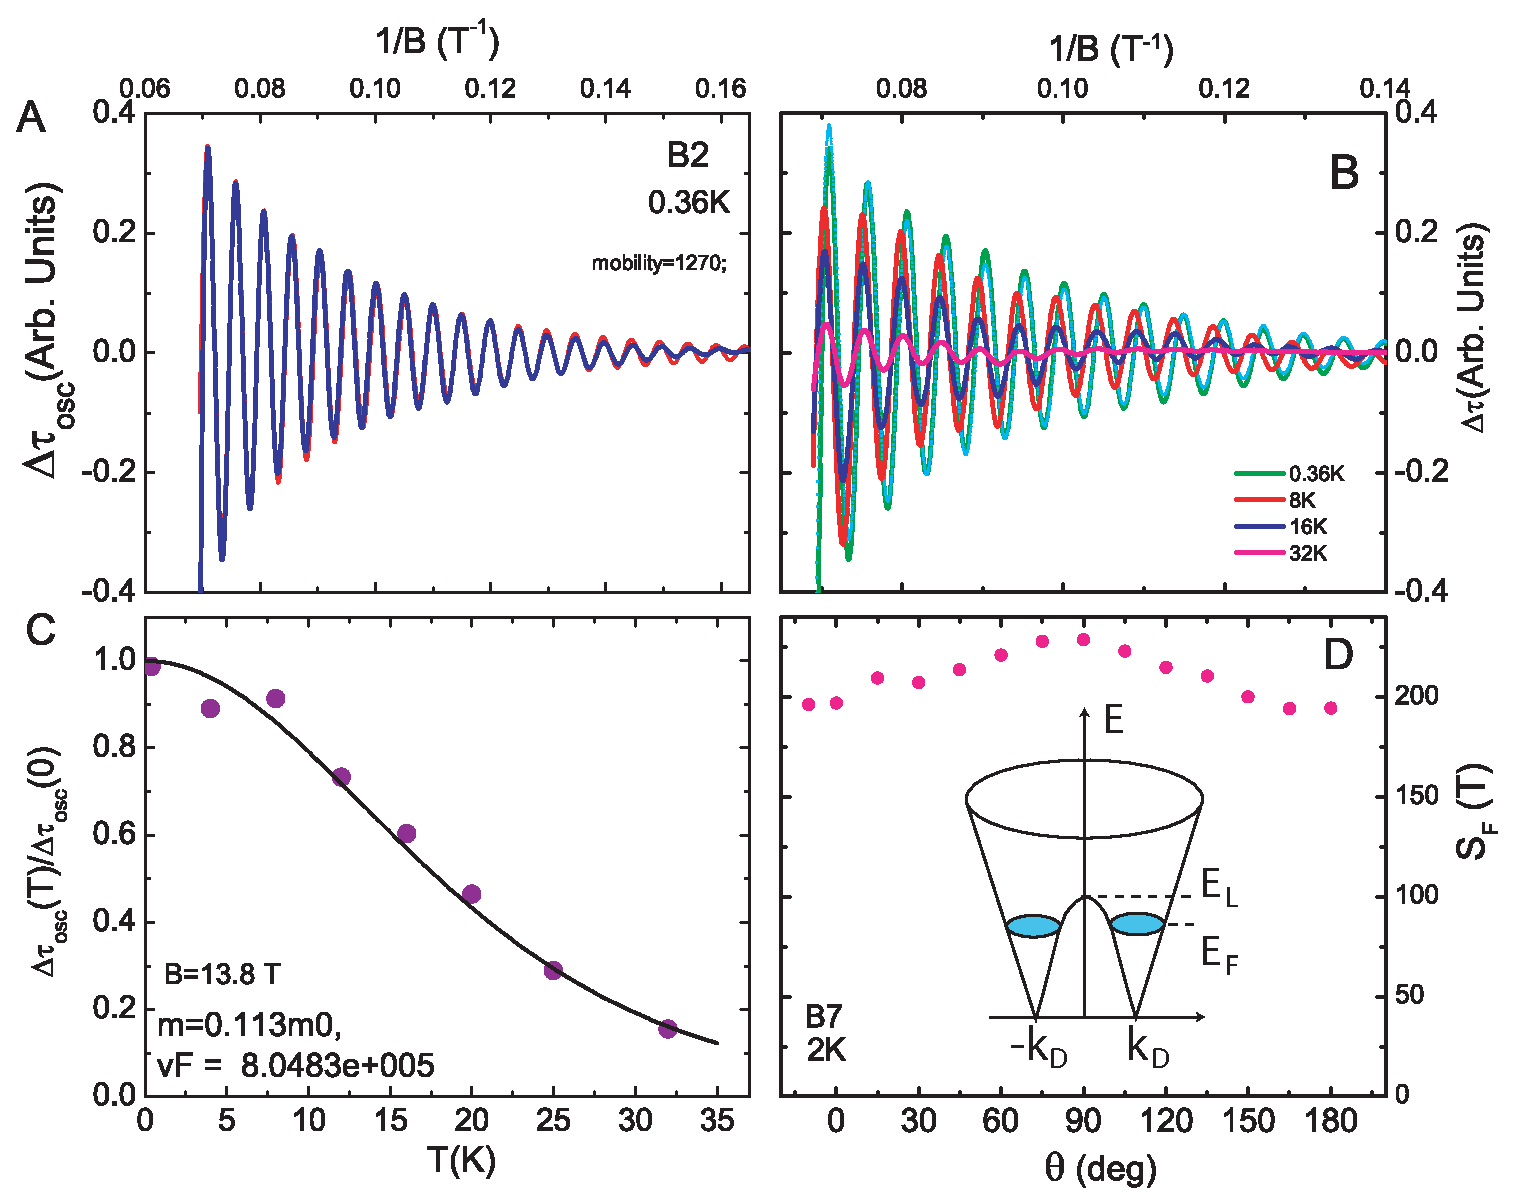
\includegraphics[width=1\linewidth]{ch-na3bi/figures/FigTorqueA}
\caption{\label{figtorque} (Color online)
Torque measurements of the de-Haas van Alven (dHvA) oscillations in Na$_3$Bi. The dHvA oscillations (solid curve in Panel A) can be fit well to the LK expression (dashed curve) with one period. From the damping versus $H$ (Panel A) and the $T$ dependence (Panels B and C), we obtain the Fermi surface section $S_F$, the effective mass $m^* = 0.11 m_0$ ($m_0$ the free mass), velocity $v_F$ = 8.05$\times 10^5$ m/s, and $\tau_Q$ = 8.16$\times 10^{-14}$s. The plot of the peak fields $B_{min}$ and $B_{max}$ vs. the integers $N$ (Panel D) yields $S_F$. 
}
  \end{center}
\end{figure}

We notice that previous Na$_3$Bi samples measured by ARPES experiments~\cite{Liu2014a, Xu2015, Xu2013} all have a chemical potential below the Dirac point. And it has hidden the information about the conduction band. In our crystals, by suppressing the Na vacancies, we have obtained crystals with $E_F$ in the conduction band, as implied by the $n$-type sign of the Hall resistivity $\rho_{yx}$. The band calculations~\cite{Wang2012} predicted the existence of two Dirac nodes centered at $(0,0,\pm k_D)$ caused by gap inversion (sketch in Fig. \ref{figtorque}D). When the energy rises following the conduction band, the two Dirac cones will eventually meet and merge into one band when the energy exceeds the Lifshitz-transition energy $E_L$. Recent ARPES experiments have confirmed the predicted dispersion and measured $k_D$ to be around 0.095 $\rm{\AA}^{-1}$~\cite{Liu2014a} and 0.10 $\rm{\AA}^{-1}$~\cite{Xu2013} (see also~\cite{Zhang2014}). But the ARPES data of the conduction band is lacked, and it cannot tell where $E_L$ is in the conduction band. An important question is whether $E_F$ in our samples lies above or below $E_L$, since $E_F$ in our sample is already quite high. We also notice that if the merged bands above $E_L$ are also isotropic, then the Fermi wave vector $k_F$ of the outer merged pocket will be larger than $k_D$ when $E_F > E_L$. On the other side, if $k_F$ is much smaller than $k_D$, then we will have  $E_F < E_L$. As shown in Table \ref{tab}, our measured $k_F$ ranges from 0.073 to 0.084 $\rm{\AA}^{-1}$. As these values are similar to but a little smaller than $k_D$, suggesting a possibility that $E_F$ lies below $E_L$. But if the merged bands are anisotropic, it's still possible that $E_F$ is slightly higher than $E_L$. This issue is worth exploring for both ARPES and transport study, and it may require crystals with a higher quality.

If $E_F < E_L$, then the FS consists of two Dirac valleys on the opposite sides of the $\Gamma$ point in the Brillouin zone, i.e. $g_v = 2$. If $E_F > E_L$, there will also be two Fermi pockets with one enclosing another. In the first case, the two Fermi surface areas will be similar but may have a small difference due to the inhomogeneity in the sample. In the second case, the two Fermi pockets will have different $S_F$, and the difference varies with $E_F$. Interestingly, We also notice that there is a persistent weak beating behavior in the SdH oscillations in many of our samples, as shown by the data of five samples in Fig. \ref{figBeats}A. Fourier transform analysis of these oscillations suggest that there are two main frequencies $f_1$ and $f_2$ corresponding to two values of $S_F$ differing by $\sim 16\%$. Such beating pattern may indicate the quantum interference between the two orbits on the two Fermi pockets. But we may need to carry out more detailed studies on such interference in the future.

\begin{figure}[!htbp]
  \begin{center}
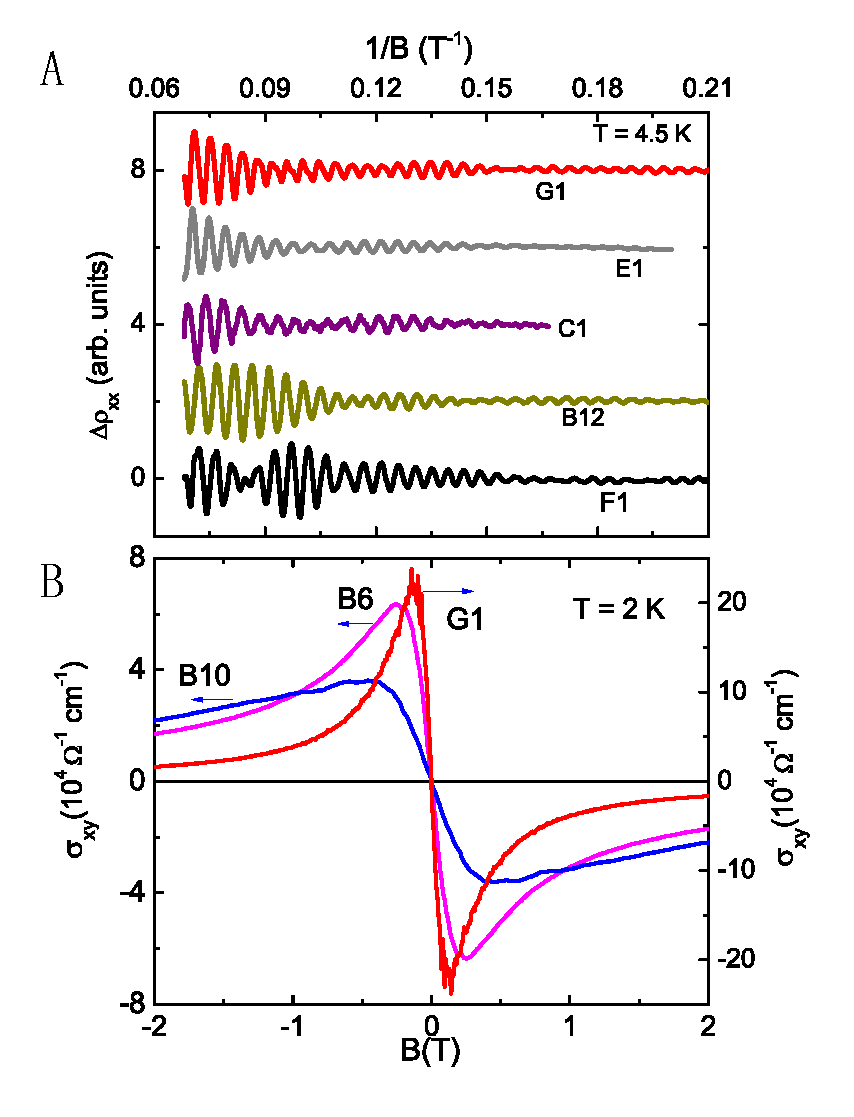
\includegraphics[width=0.9\linewidth]{ch-na3bi/figures/FigBeatsDrude.pdf}
\caption{\label{figBeats} 
Panel A: Curves of $\Delta\rho_{xx}$ showing modulation of the SdH amplitudes in different Na$_3$Bi samples. The beating pattern implies a small splitting of the fundamental SdH frequency.
Panel B compares the Hall conductivity $\sigma_{xy}(B)$ in 3 samples at 2 K. In the 3 curves, the peak field $\pm B_{\mu}$ yields the values $\mu$ = 21,640, 39,250 and 91,000 cm$^2$/Vs in B10, B6 and G1, respectively.
}
  \end{center}
\end{figure}

As reported in \cite{Liang2015}, there could be a strong suppression of backscattering in Dirac semimetals. Therefore it is of great value to investigate both the transport lifetime $\tau_{tr}$ and the quantum lifetime $\tau_Q$ in Na$_3$Bi. The conventional way to obtain $\tau_{tr}$ is from the ratio of $\rho_{yx}/\rho_{xx}$, but it requires very accurate measurement of sample dimensions. Since we mount our Na$_3$Bi samples in the glove box and the thickness measurement is not accurate, the calculated $\tau_{tr}$ by this method will have a large error bar. Instead, we leverage the Drude formula for $\sigma_{xy}$ to find $\tau_{tr}$. By the Bloch-Boltzmann theory, the extrema in $\sigma_{xy}(B)$ occur at the peak fields $\pm B_\mu$, where $1/B_\mu$ equals the ``Hall mobility'' $\mu_H$. Fig. \ref{figBeats}B shows the typical $\sigma_{xy}(B)$ curves of three samples which have the characteristic dispersion-resonance profile produced by cyclotron motion of the carriers. The $\sigma_{xy}(B)$ curves are derived by inverting the measured resistivity matrix $\rho_{ij}(B)$. As displayed in Fig. \ref{figBeats}B, the mobilities from Sample B10 ($\mu$ = 21,640 cm$^2$/Vs) to B6 (39,250 cm$^2$/Vs) and G1 (91,000 cm$^2$/Vs), increase as the peak field $B_{\mu}$ decreases. We will discuss below the influences on the Hall angle profiles from different $\mu_H$. With $\mu = ev_F\tau_{tr}/\hbar k_F$, we find that the transport lifetime $\tau_{tr}$ exceeds $\tau_Q$ by a ratio $R_{\tau}$ = 10-20 ($R_{\tau}$ is expected to exceed 1 since $\tau_Q$ reflects broadening due to all scattering processes). As a comparison, $R_{\tau}$ in Cd$_3$As$_2$ is as large as 10$^4$~\cite{Liang2015}. 




%In the relaxation-time $\emph{ansatz}$, the Boltzmann equation describing changes to the distribution function $f_{\bf k}$ caused by an electric 
With the relaxation-time approximation, the Boltzmann equation that describes the change of the distribution function $f_{\bf k}$ in an electric 
field $\bf E$ is expressed as~\cite{Ziman}
\be
e{\bf E\cdot v}\frac{\partial f^0_{\bf k}}{\partial E_{\bf k}}  
+ e{\bf v\times B\cdot}\frac{\partial g_{\bf k}}{\partial {\bf k}}
= -\frac{g_{\bf k}}{\tau_{tr}},
\label{Boltz}
\ee
where $e$ is the elemental charge and $g_{\bf k} = f_{\bf k}-f^0_{\bf k}$, with $f^0_{\bf k}$ the Fermi-Dirac function. $E_{\bf k}$ and the velocity $\bf v$ are, respectively, the energy and velocity at state $\bf k$. Then the conductivity tensor $\sigma_{ij}$ is
\be
\sigma_{xx} = ne\mu/D, \quad\quad \sigma_{xy} = ne\mu^2B/D,
\label{sxx}
\ee
where $D = 1+(\mu B)^2$. We notice that the ratio $\sigma_{xy}/\sigma_{xx}= \mu B$, which is the Hall angle $\tan\theta$, is linear in $B$. When the conductivity matrix is converted to the resistivity matrix, the above $\emph{ansatz}$ yields a $B$-independent $\rho_{xx}$. This is because the Hall electric-field $E_y$ exactly balances the Lorentz force. Moreover, we can obtain $\sigma_{xx}\sim 1/B^2$ and $\sigma_{xy}\sim 1/B$ at large $\mu B$. In a material that has two types of carriers with different mobilities, $\rho_{xx}$ will follow a $B^2$ dependence at low fields and will saturate at high fields. The key assumption underlying these standard predictions is that $\tau_{tr}$ (hence $\mu$) is a constant independent of $B$. This assumption has been firmly established in conventional metals and semimetals in the impurity-scattering regime (elastic scattering). The prediction is a cornerstone of semiclassical transport.


Nevertheless, the observed field dependences of $\sigma_{xx}$ and $\rho_{xx}$ in Na$_3$Bi follow an essentially different profile from the standard predictions while only $\rho_{yx}(B)$ appears conventional. As shown in Fig. \ref{figR}, $\rho_{xx}$ in Na$_3$Bi increases linearly with $B$ without any saturation. In B11 (Fig. ref{figMRtan}), we show that the $B$-linear profile extends to 35 T with no evidence of deviation or saturation. This behavior deviates from the predicted quadratic field dependence. A $B$-linear MR is rare in conventional conductors (see Abrikosov's comments~\cite{Abrikosov1998}. Sometimes it can be caused by open orbits. But here we can exclude the possibility of open orbits~\cite{Ziman}). However, interestingly, there are increasing numbers of examples for a $B$-linear MR in materials with unusual topological phases~\cite{Qu,Liang2015}. To find out whether the $B$-linear MR is universal in Na$_3$Bi crystals with high $E_F$, we have investigated eight samples (Table \ref{tab}). All these samples have a similar MR profile. Figure \ref{figMRtan}A shows that the $B$-linear MR is a very robust feature in Na$_3$Bi. We also notice that the MR ratio (measured at 15 T) could be very different among our samples, as it increases from $\sim 14$ in B10, to $163$ in G1 (the sample with the highest $\mu$). A more detailed test of the correlation between the MR ratio and the sample mobility will be made in the future. 



We also find a dramatic anomaly in the Hall-angle profile. In Fig. \ref{figMRtan}B, we compare the $\tan\theta$ v.s. $B$ curves measured in four samples with an increasing $\mu$, i.e. B10, B12, B6 and G1. In all these samples, $\tan\theta$ initially rises very rapidly in weak $B$ and then saturates to a value independent on the magnetic field. Besides, the slope of the rise at low $B$ depends on the mobility. The samples (B10 and B12) with a low $\mu$ have a gentle rise in $\tan\theta$ while the samples (B6 and G1) with a high $\mu$ have an abrupt rise. In particular, the $\tan\theta$ v.s. $B$ curve in Sample G1 resembles a step function. Since $\tan\theta = \mu B$, if we assume that $\tan\theta$ in Na$_3$Bi has a universal independent behavior starting at weak fields (B$>$0.5 T), then a simple explanation will be a decreasing $\tau_{tr}$ with the increasing B, such as 
\be
\tau_{tr} \sim 1/B.
\label{tau}
\ee



We also notice that Eq. \ref{tau} could also account for the $B$-linear MR profile, i.e. 
$\rho_{xx} = 1/ne\tau_{tr} \sim B.$
Interestingly, Eq. \ref{tau} implies that the high-field $B$ dependence of $\sigma_{xx}$ is reduced by one power of $B$ to $\sigma_{xx}(B)\sim 1/B$ (Eq. \ref{sxx}), but does not modify the field dependence of $\sigma_{xy}$ ($\sigma_{xy}\sim 1/B$). This is because $\mu$ cancels out at large $B$. Therefore both $\sigma_{xx}$ and $\sigma_{xy}$ evolve as $1/B$ at large $B$, generating the step-profile of $\tan\theta$. 

\begin{figure}[!htbp]
  \begin{center}
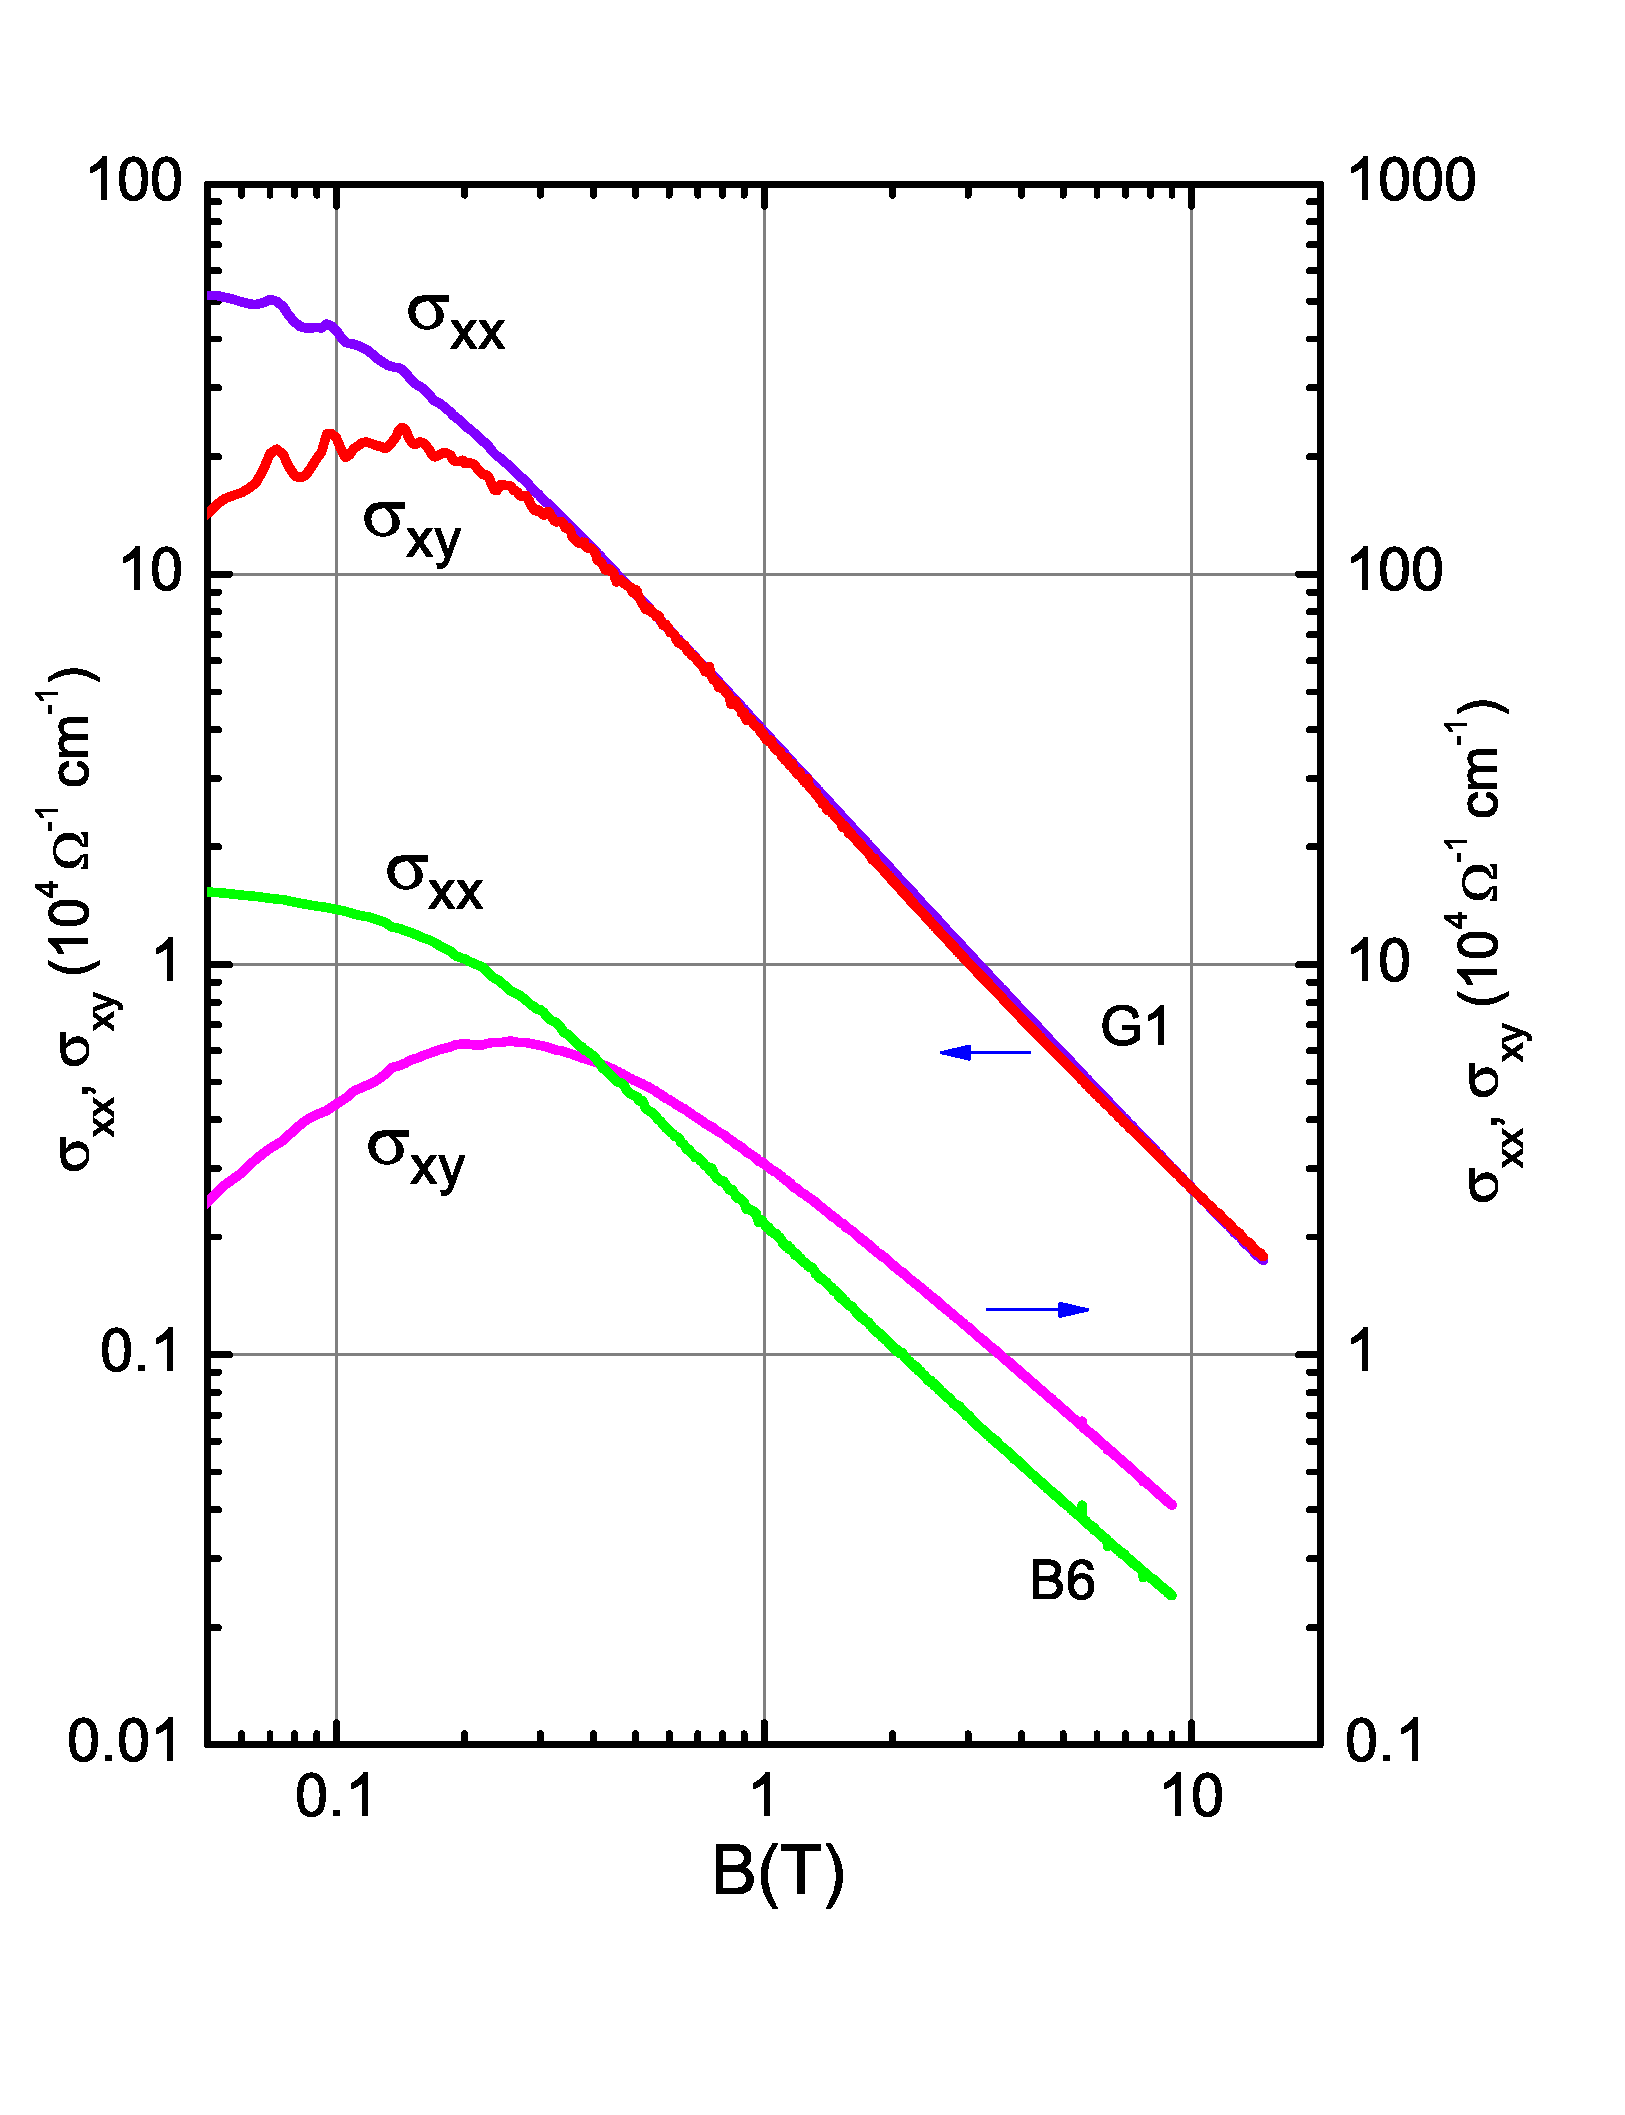
\includegraphics[width=0.8\linewidth]{ch-na3bi/figures/FigLogSigxy}
\caption{\label{figCond} 
Log-log plots of $\sigma_{xx}$ and $\sigma_{xy}$ vs. $B$ in Sample G1 and B6. Consistent with Eq. \ref{tau}, both quantities approach the same power law $B^{-\beta}$ when $B$ exceeds 0.3 and 2 T in G1 and B6, respectively. The measured $\beta$ is 1.15 and 1.0 in G1 and B6, respectively. Curves for B6 are shifted vertically.
}
  \end{center}
\end{figure}



\begin{figure}[!htbp]
  \begin{center}
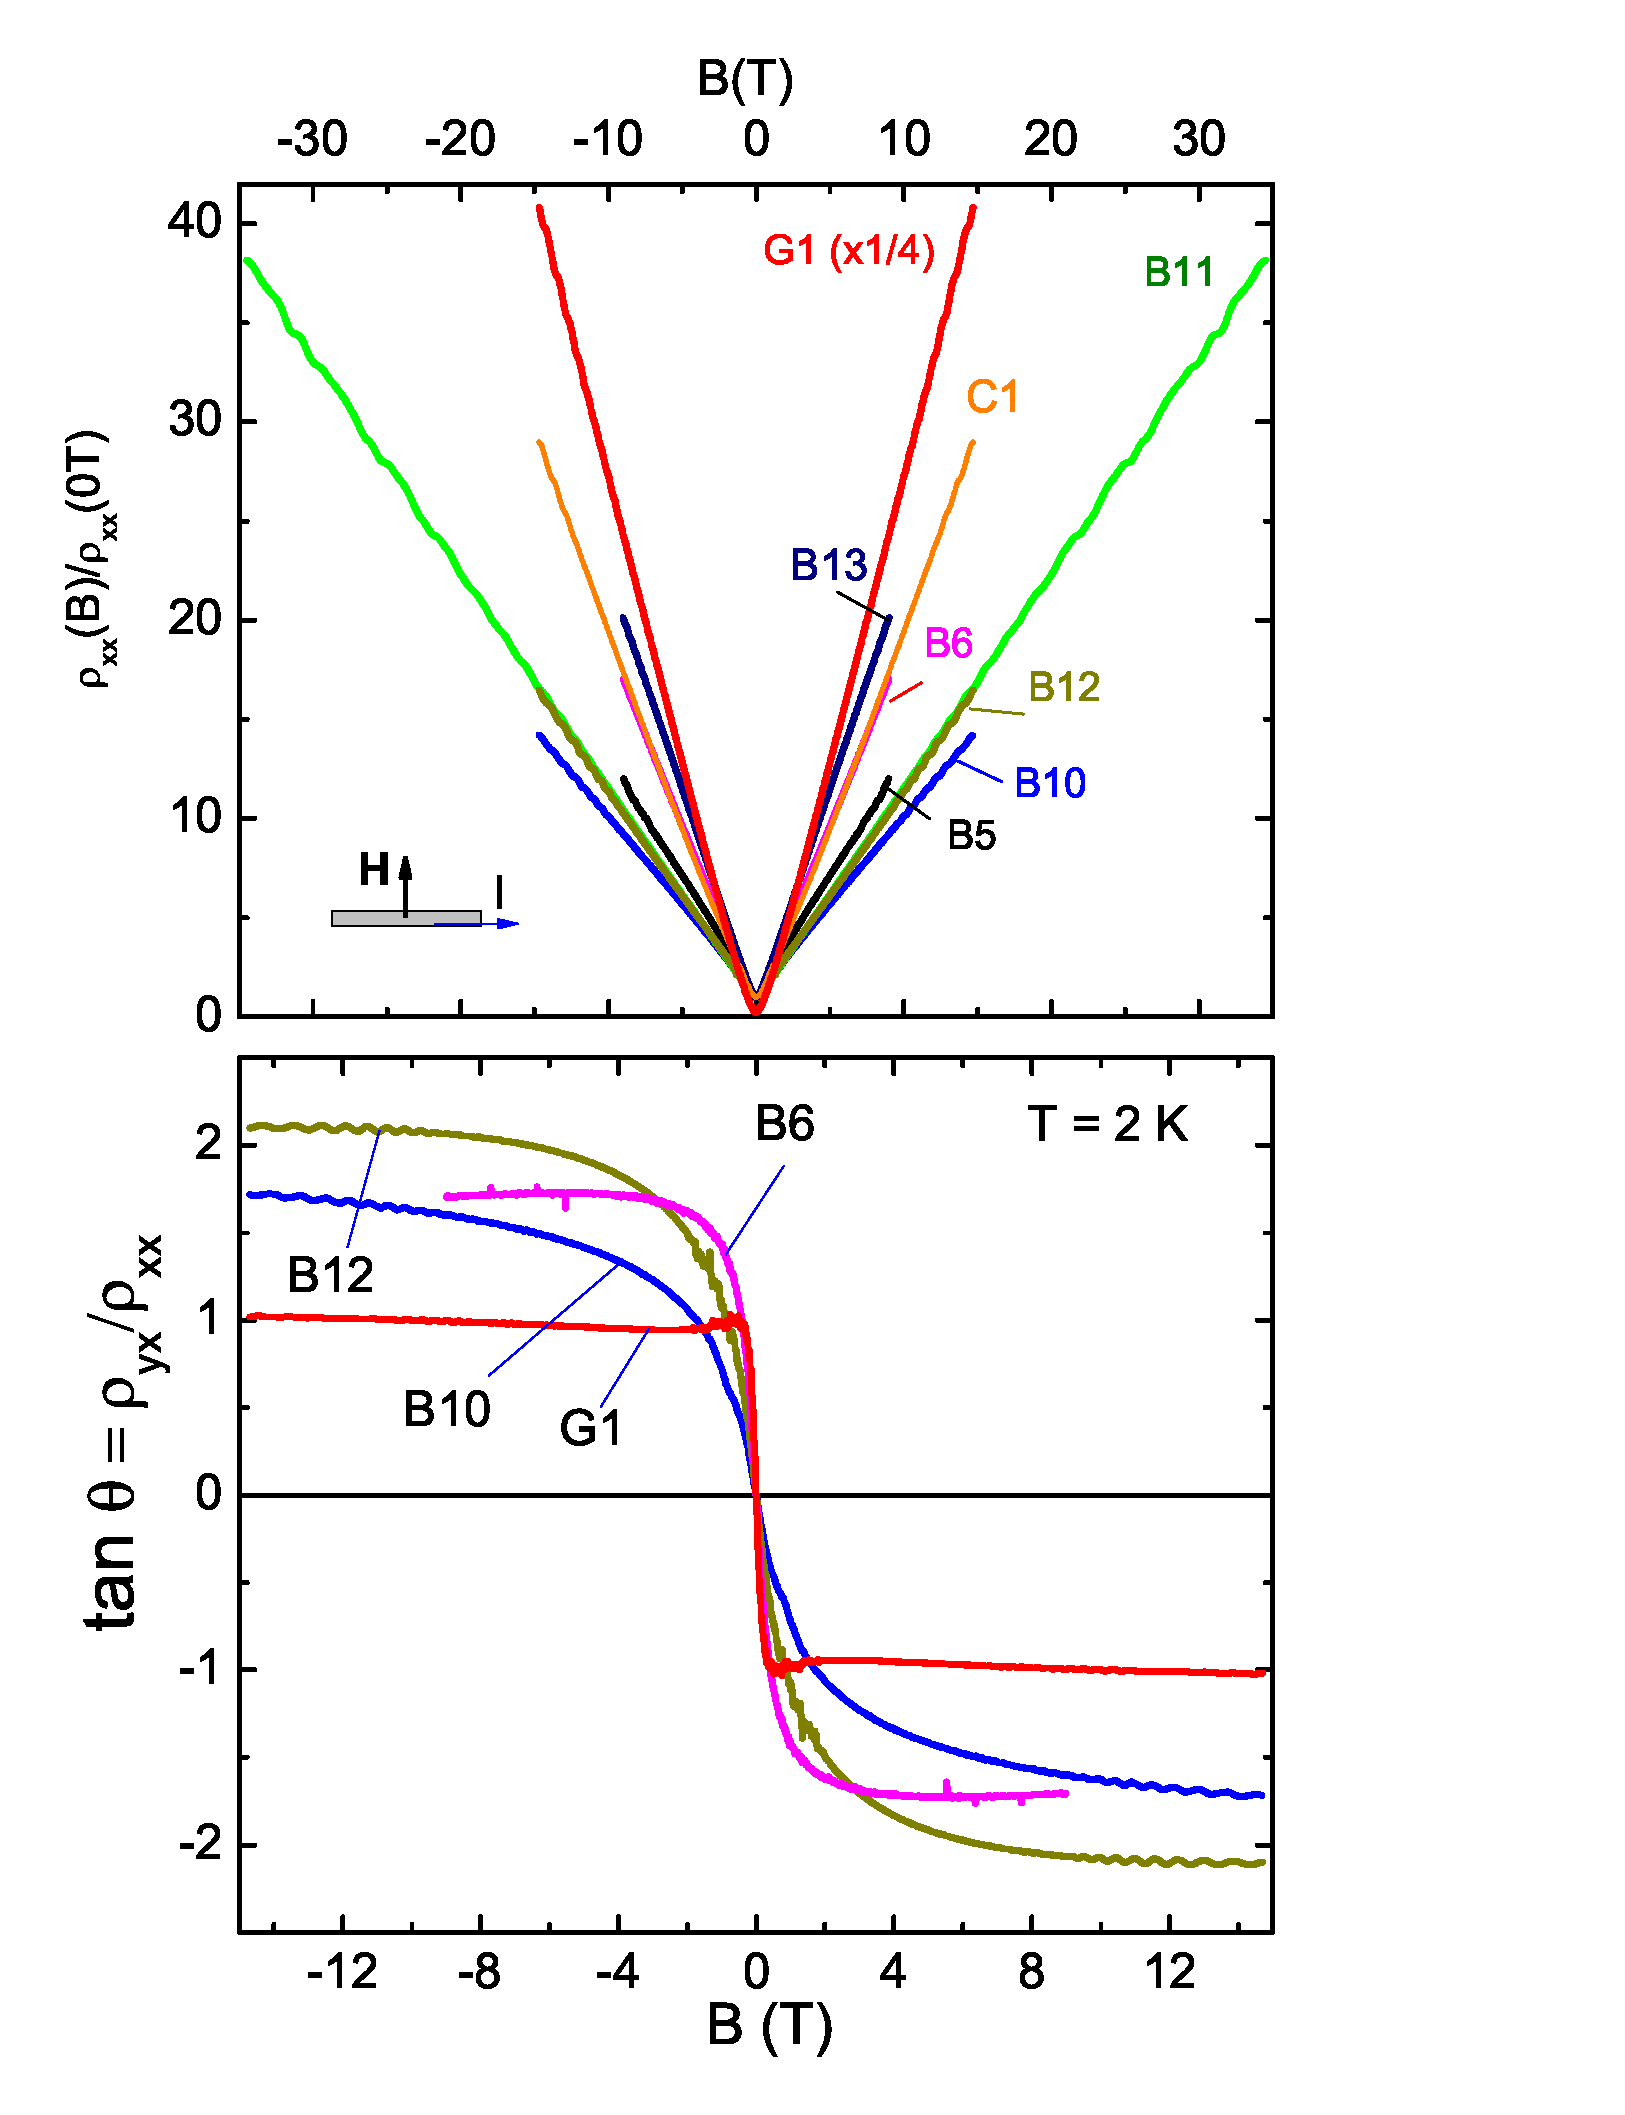
\includegraphics[width=0.9\linewidth]{ch-na3bi/figures/FigMRHallAngle}
\caption{\label{figMRtan}
Robust $H$-linear magnetoresistance in Na$_3$Bi (Panel A). In the 8 samples displayed here, $\rho_{xx}(B)$ is measured with $\bf H||\hat{c}$ at 2 K in all cases except in B11 (at 1.6 K). In B11, the MR persists without observable deviation to 35 T. A general trend is that the MR increases with $\mu$, from $\sim 14$ (at 15 T) in B10, to $\sim 160$ in G1 (which has the highest $\mu$) (the MR in G1 is plotted in $\frac14$ scale). In Panel B, the field profile of $\tan\theta = \rho_{yx}/\rho_{xx}$ is compared in 4 samples. As $H$ increases, $\tan\theta$ rapidly saturates to an $H$-independent value, which implies the anomalous relationship $\tau_{tr}\sim 1/H$. In G1, the change occurs at 0.5 T.}
  \end{center}
\end{figure}


To verify the above speculation on the same power law behavior of $\sigma_{xx}$ and $\sigma_{xy}$, we plot the $B$ dependences of $\sigma_{xx}$ and $\sigma_{xy}$ in log-log scale for the two high-mobility samples B6 and G1 (Fig. \ref{figCond}). The same slope of both of $\sigma_{xx}$ and $\sigma_{xy}$ in both samples indicates the same power-law dependence $B^{-\beta}$ at high fields. Compared with the starting field for the saturation of $\tan\theta$, we find that starting field of the same power-law dependence is also at $B$ = 2 T and 0.3 T in B6 and G1 respectively. This consistency provides a reasonable support for our explanation. We also notice that the measured value of $\beta$ is 1.0 in B6, but is slightly larger (1.15) in G1. 



%We will also compare the behavior of Na$_3$Bi and Cd$_3$As$_2$.





%%%%%%%%%%%%%%%%%%%%%%%%


%%%%%%%%%%%%%%%%%%%%%%%%%%%
%%%%%%%%%%%%%%%%%%%%%%%%%%%
%%%%%%%%%%%%%%%%%%%%%%%%%%%
%\vspace{3cm}
%
%\newpage

%%%%%%%%%%%%%%%%%%%%%%%%%%%%%%%%%%
%%%%%%%%%%%%%%%%%%%%%%%%%%%%%%%%%%
%%%%%%%%%%%%%%%%%%%%%%%%%%%%%%%%%% FIGURE 1




%%%%%%%%%%%%%%%%%%%%%%%%%%%%%%%%%%
%%%%%%%%%%%%%%%%%%%%%%%%%%%%%%%%%%
%%%%%%%%%%%%%%%%%%%%%%%%%%%%%%%%%% FIGURE 2

%%%%%%%%%%%%%%%%%%%%%%%%%%%%%%%%%



%%%%%%%%%%%%%%%%%%%%%%%%%%%%%%%%%%
%%%%%%%%%%%%%%%%%%%%%%%%%%%%%%%%%%
%%%%%%%%%%%%%%%%%%%%%%%%%%%%%%%%%% FIGURE 3

%%%%%%%%%%%%%%%%%%%%%%%%%%%%%%%%%%


%%%%%%%%%%%%%%%%%%%%%%%%%%%%%%%%%%
%%%%%%%%%%%%%%%%%%%%%%%%%%%%%%%%%%
%%%%%%%%%%%%%%%%%%%%%%%%%%%%%%%%%% FIGURE 4

%%%%%%%%%%%%%%%%%%%%%%%%%%%%%%%%%%


%%%%%%%%%%%%%%%%%%%%%%%%%%%%%%%%%%
%%%%%%%%%%%%%%%%%%%%%%%%%%%%%%%%%%
%%%%%%%%%%%%%%%%%%%%%%%%%%%%%%%%%% FIGURE 5

%%%%%%%%%%%%%%%%%%%%%%%%%%%%%%%%%%

%\newpage
\hfill \break

\begin{table*}[!htbp]
  \begin{center}
\begin{tabular}{|c|c|c|c|c|c|c|c|c|} \hline
Sample	& $\rho$(4 K)       & $n_H$	& $k_F$ &     $n_F$       &  $\mu'$    &     $\mu$  & MR(9 T)  & $\tau_{tr}$ \\ \hline
(units)   & $\;\;\mu\Omega$cm$\;\;$ & $10^{19}$ cm$^{-3}$  &  $\rm{\AA}^{-1}$    &   $10^{19}$ cm$^{-3}$      &  cm$^2$/Vs      & cm$^2$/Vs  & --  & ps \\ \hline\hline
B5		  &	34         &			  --      &	  0.083		 &  3.8      &     	--    &   --		         &    5.69   &   -- \\ \hline
B6		  &  6.2		        &   2.9		&   0.079		 &  	3.4     &		35,000    &   39,200    &  17     &   2.55 \\ \hline
B10	  &  7.5				   &  6.5				& 	0.081      &		3.6    &    13,000    &  	21,600  & 9.62   &  1.49  \\ \hline
B11	  &  87        &  1.3				&  0.073			&  	2.6 			&  5,500        &     --        &  10.5  &  --  \\ \hline
B12	  &  7.4        &  3.7				&  0.082			&  	3.7 			&  23,000        &  27,900  &    10.3 &  1.94 \\ \hline
C1			&  5.1					&  8.9				&  0.084			&   4.0			&  13,600      &   26,500    & 16.2  &  1.93  \\ \hline
F1	      &  6.6         &  6.5         &  0.082     &   3.7     &   14,600     &   30,400   &  32.8  &  2.11  \\  \hline
G1			&  1.72					&  4.6					&  0.085		&   4.1			&  78,900	   &   91,000   & 97.1   &   6.71 \\ \hline
\end{tabular}
\caption{\label{tab}
Transport parameters in 8 samples of Na$_3$Bi. $n_H$ is the Hall density inferred from $R_H$. $k_F$ is the FS wavevector inferred from the period of the quantum oscillations and $n_F = g_vk_F^3/3\pi^2$ with $g_v =2$. $\mu'$ is the transport mobility derived from $\rho$(4 K) and $n_F$, while $\mu$ is directly read from the profile of $\sigma_{xy}(B)$ in Fig. 3B (main text). MR(9 T) is the MR ratio measured at 9 T. $\tau_{tr}$ is calculated from $\mu = ev_F\tau_{tr}/\hbar k_F$. The quantities $\rho$, $n_H$ and $\mu$ are subject to the large uncertainty in estimating $t$ ($\pm 50\,\mu$m), but $k_F$, $n_F$ and $\mu_H$ are unaffected. F1 and G1 were post-annealed for 2 weeks and 1 month, respectively. The quantities $\rho$(4 K) and $n_H$ are strongly affected by the large uncertainty in $t$, but $k_F$, $n_F$, $\mu$ and $\tau_{tr}$ are not.
}
  \end{center}
\end{table*}




As described above, the observed transport properties of Na$_3$Bi are unexpected, and may need further and systematic theoretical study of the transport theory on Dirac semimetals. The Dirac semimetal may be regarded as the limiting case when TRI is present and the paired Weyl nodes coincide at the same point in $\bf k$ space, protected by the crystalline symmetry. As a result, the Berry curvature generated by different Weyl nodes annihilates. When TRI is broken in a magnetic field, the Berry curvature $\vec{\Omega}(\bf k)$ will appear and evolve as the B increases. Therefore, the FS topology may be changed in a magnetic field, and may lead to the unconventional behavior of  $\sigma_{xx}$ and $\rho_{xx}$ in transport experiments. But to completely understand this effect, there needs to be more specific theory that addresses the evolution of FS and scattering time in a high magnetic field.